\documentclass[onecolumn, draftclsnofoot,10pt, compsoc]{IEEEtran}
\usepackage{graphicx}
\usepackage{url}
\usepackage{setspace}
\usepackage{times}
\usepackage{enumitem}
\usepackage{titletoc}
\usepackage{float}
\usepackage{listings}
\usepackage{caption}
%\usepackage[export]{adjustbox}
%\usepackage[notocbib]{apacite}
\usepackage{geometry}
\geometry{textheight=9.5in, textwidth=7in}

% 1. Fill in these details
\def \CapstoneTeamName{		Beached Marine Critters Project Team}
\def \CapstoneTeamNumber{		64}
\def \GroupMemberOne{			Alea Weeks}
\def \GroupMemberTwo{			Amar Raad}
\def \GroupMemberThree{			Daniel Domme}
\def \GroupMemberFour{			Justin Disalvo}
\def \GroupMemberFive{			Zachary Tusing}
\def \CapstoneProjectName{		Develop a visual model for sea turtle beach stranding Events}
\def \CapstoneSponsorCompany{	Oregon State University Hatfield Marine Science Center; Oregon Sea Grant}
\def \CapstoneSponsorPerson{		Dr. William Hanshumaker}

% 2. Uncomment the appropriate line below so that the document type works
\def \DocType{		%Problem Statement
				%Requirements Document
				%Technology Review
				%Design Document
				Progress Report
				}
			
\newcommand{\NameSigPair}[1]{\par
\makebox[2.75in][r]{#1} \hfil 	\makebox[3.25in]{\makebox[2.25in]{\hrulefill} \hfill		\makebox[.75in]{\hrulefill}}
\par\vspace{-12pt} \textit{\tiny\noindent
\makebox[2.75in]{} \hfil		\makebox[3.25in]{\makebox[2.25in][r]{Signature} \hfill	\makebox[.75in][r]{Date}}}}
% 3. If the document is not to be signed, uncomment the RENEWcommand below
\renewcommand{\NameSigPair}[1]{#1}
\doublespacing
%%%%%%%%%%%%%%%%%%%%%%%%%%%%%%%%%%%%%%%
\begin{document}
\begin{titlepage}
    \pagenumbering{gobble}
    \begin{singlespace}
     \includegraphics[height=3cm]{coe_v_spot1}
        \hfill 
        % 4. If you have a logo, use this includegraphics command to put it on the coversheet.
        %\includegraphics[height=4cm]{CompanyLogo}   
        \par\vspace{.2in}
        \centering
        \scshape{
            \huge CS Capstone \DocType \par
            {\normalsize\today}\par
            \vspace{.5in}
            \textbf{\Huge\CapstoneProjectName}\par
            %\vfill
            \vspace{1in}
            %{\Large Prepared for}\par
            %\huge \CapstoneSponsorCompany\par
            %\vspace{5pt}
            % {\Large\NameSigPair{\CapstoneSponsorPerson}\par}
            % \vspace{.5in}
            {\large Prepared by }\par
            Group\CapstoneTeamNumber\par
            % 5. comment out the line below this one if you do not wish to name your team
            %\CapstoneTeamName\par 
            \vspace{5pt}
            {\Large
                \NameSigPair{\GroupMemberOne}\par
                \NameSigPair{\GroupMemberTwo}\par
                \NameSigPair{\GroupMemberThree}\par
				\NameSigPair{\GroupMemberFour}\par
			\NameSigPair{\GroupMemberFive}\par
            }
            \vspace{20pt}
        }
        \vfill
        \begin{abstract}
        % 6. Fill in your abstract    
        	%This document is written using one sentence per line.
        	%This allows you to have sensible diffs when you use \LaTeX with version control, as well as giving a quick visual test to see if sentences are too short/long.
        	%If you have questions, ``The Not So Short Guide to LaTeX'' is a great resource (\url{https://tobi.oetiker.ch/lshort/lshort.pdf})
		    \noindent This document is a summary of all activities that took place during this term and the current state of the project. The outline of problems, possible solutions, and learned is also discussed. 
		    
        \end{abstract}     
    \end{singlespace}
\end{titlepage}
\newpage
\pagenumbering{arabic}
\tableofcontents
% 7. uncomment this (if applicable). Consider adding a page break.
\listoffigures
%\listoftables
\clearpage
%\begin{singlespace}

\section{Project Purpose and Goals}
The purpose of the beached marine critters project is to use archival data to create a visual model of sea turtle beach stranding events. The archival data will include information about the beached animal as well as sea conditions such as sea surface temperature, currents and wind direction. The ultimate purpose is to use the visual model to draw correlations between preexisting ocean conditions and the dates of sea turtle stranding events. The goal is to gain understanding of how oceanographic conditions lead to stranded animals aid in the timely rescue of sea turtles.

\section{Current State of Project}
\subsection{ArcGIS and Data Collection}
We have made good progress on creating a visual representation of stranded sea turtle and sea condition data.
We have gathered historical data from the years 1957 - 2018 on sea conditions for the Pacific Northwest Coast\cite{noaa}. The data has more than 4 million unique rows representing historical weather data for each day from the year 1957 until 2018. We will use this data to calculate daily averages of wind direction and speed to create a map layer. The data are standardized to match the format of the beached sea turtle data. Additionally, sea surface temperatures and air temperatures were gathered from NOAA\cite{sst}\cite{rest} (National Oceanographic and Atmospheric Administration) in formats that are readily usable in our project. Marine current data has been gathered\cite{jpl}, but there is a mismatch in latitude and longitude formats.  We are looking for a solution to the problem.


We have imported the sea turtle data into ArcGIS (mapping and data analysis software) and have visually represented this data on the map. This is shown in Figure 1. \newline \newline

\begin{figure}[H]
  \includegraphics[scale=0.55]{turtle_data.eps}
  \caption{Sea turtle data plotted on a map}
\end{figure}

The next couple of screenshots give examples of how our sea condition data looks when overlapped. Figure 2 shows the daily averages for sea surface temperature from June 30, 1993 - July 1, 1993. The daily average sea surface temperature is shown as the colored gradient layer with blue colors representing colder temperatures and yellow/orange colors representing hotter temperatures. Figure 2 also has wind vectors that represented daily averages for wind direction and speed. Smaller vectors with lighter colors represent weaker winds. Larger vectors with darker colors represents stronger winds. Additionally, Figure 2 has 2 sea turtle stranding events, indicated by the light green hexagons. This means that between June 30, 1993 and July 1, 1993, two sea turtles were found at the areas shown on the map. The specific sea turtle species are labeled next to the points. \newline

\begin{figure}[H]
  \includegraphics[scale=0.40]{wind_and_sst_93.eps}
  \caption{Wind velocity and sea surface temperature map layers}
\end{figure}

Figure 3 shows the same wind and turtle data as Figure 2. However, Figure 3 has daily air temperature averages shown, represented by the colored gradient layer. 

\begin{figure}[H]
  \includegraphics[scale=0.4]{air_temp_and_wind_93.eps}
  \caption{Wind velocity and air temperature map layers}
\end{figure}



\subsection{Graphical User Interface (GUI)}
The project's user interface (UI) needed to provide simple functionalities and be easily manipulable for the rest of our team. The UI was designed with simplicity in mind so that researchers and inexperienced users would easily be able to understand what is going on. The UI has simple button outline for easy access to our different functions. We've been working to provide a larger base of functionality most of the term so that the rest of the team can start working on the background functions and implementing them for the GUI. We are not satisfied with the look of the GUI and are intending to provide a better look and feel to everything about our UI. This means that we will provide a simple yet beautiful GUI.

\subsection{Integration}

Upon complete integration, the recorded locations of sea turtle stranding events should be able to display on the map implemented into the GUI. Selecting "From" and "To" timestamps should then call for the time period of all recordings found in-between the two. When calling for this function, the GUI should access and retrieve data from the ArcGIS map, selecting the appropriate data to be displayed for the user. Although the integration between the ArcGIS map and GUI is still in process, once the GUI can successfully pull and display data from a static timestamp of data, then toggling along different timestamps with the live data should be next to implement.

\section{What Needs to Be Done}

\subsection{ArcGIS and Data Collection} 
\par NetCDF files for air temperature and sea surface temperature need to be combined together to make adding data layers to the map easier.  If the files become too large, however, ArcGIS will struggle with loading it all properly.  File sizes need to be considered when this happens.  One gigabyte will be considered the cutoff size for files.
\par The ocean current data needs to be standardized to make vectors on the map.  The format that it is currently in will not work effectively.

\par Visually there is a lot of little improvements we still need to make to the map. For example, in Figures 2 and 3 a lot of sea condition data has been interpolated and includes average sea data on land. To fix this we need to limit the sea condition data to only be plotted on sea and not on land. Other visual improvements will be made after our client reviews our work and provides feedback. 

\subsection{Graphical User Interface (GUI)}
\par So far, the GUI is very basic. All the buttons are present, and the structure is complete. All that is left is making it look nicer and making any changes that may need to be made based on the integration of ArcGIS. One of these changes will be the Data section to the right of the map. This will be created based on the number of sea turtles that are in the imported file.
\begin{figure}[H]
  \includegraphics[scale=0.6]{current-ui.eps}
  \caption{Current State of the GUI}
\end{figure}
\subsection{Integration}
The integration is where much of the team is focusing their time. Due to the struggle that it has been to bridge the PyQT GUI with ArcGIS. The GUI is currently being looked at as a target of restructuring, since there seems to be limited ways to make a portable executable file with PyQT and ArcGis. The team has been looking at introducing a conversation file from PyQT to QT. QT has a CPP transition file to convert any PyQT to QT or vice-versa. Therefore the team is looking at moving into the CPP space to better integrate with our ArcGIS back end. This new ArcGIS back end would be working with ArcEngine, which is a development package for ArcGIS. This will allow the team to deliver the executable package. and meet the requirements from our requirements document. The team needs to make a decision on if there is a need to move forward with this implementation process. Currently, it seems to be the route the team will take.


\section{Problems and Solutions}
\subsection{ArcGIS and Data}
During the initial weeks of this term, multiple members of the team had problems getting access to ArcGIS software license. 

\par A roadblock that was faced by the team in gathering data from government sources early in the term was the government shutdown.  Many agencies that collected and published data sets for weather and sea conditions were not operating. The websites were not accessible for a few weeks.  This caused a disruption in the amount of work that could be done with processing and mapping data.  Fortunately, after the shutdown ended, the websites were operational again, and the necessary data could be gathered.

A problem that we had with the data for our project is that the amount of weather data that was collected was immense in volume.  There were over 54 million unique lines of weather entries.  This posed a problem with the stability of the ArcGIS software, which, when overloaded with computations, crashes or slows down to unusable speeds.  The solution to this was to process the data in multiple steps.  The first step was to average data points that were close together in latitude and longitude.  Any points that were within three degrees of each other on the same day were combined.  This helped to reduce data by 40\% to 32 million entries.  This was still too much, so the data was processed again.  Every tenth entry was put into a new file.  This still maintained enough data for plotting data, yet it was manageable enough for ArcGIS to work with it.  It brought data lines down to around six million lines.

Another data problem that is currently being faced is with the ocean currents historical data. The data set we have is called OSCAR (Ocean Surface Current Analysis Real-time)\cite{jpl} from NASA Jet Propulsion Laboratory. It is the most complete, well documented, and applicable data set for ocean currents that we've been able to find. The data is in netCDF format (a file format that is used to plot weather data in mapping software) which is what needed in order to make multidimensional raster layers (file that are multidimensional in format to make relationships between types of data) in ArcGIS. The only problem with this data set is that it uses a different coordinate system than the rest of our data. This means when it is plotted in ArcGIS, the ocean currents data is heavily shifted to the right of where it should be. This is shown in Figure 4. Figure 4 shows how the ocean currents data does not match up with the map and the rest of the data. To fix this, the netCDF files will have to be edited in order to change the coordinate system to that of the rest of the data. It is not currently known if this is possible.

\begin{figure}[H]
  \includegraphics[scale=0.4]{currents_problem.eps}
  \caption{Ocean Currents Data}
\end{figure}

\subsection{Graphical User Interface (GUI)}
The code to make the GUI is very confusing. We used QtDesigner to create it, and it automatically converts it to a python file. Going through the code and properly commenting and spacing it out will help everyone understand it better. Next, is addressing the Data portion to the right of the map. This will be created when the file is imported. A button will be created for each point on the map, and will be linked to highlight the point on the map when clicked.
\subsection{Integration}
There still is a roadblock in accessing our ArcGIS database. Initially, I also had difficulties acquiring a full licence to the ArcGIS software, so any testing was done with public example maps and locations. However, I was recently able to obtain assistance in acquiring the needed access so I will be able to view and test the integration with a static set of data.

\section{Interesting Code}
\subsection{ArcGIS and Data}
Much of the weather data that was collected from NOAA was in the form of lines of data that had too much information, and it was not very intuitive. In addition, there was data for locations that were not important to our project. It needed to be filtered and transformed.  Data files for multiple daily measurements from 1957 until 2018 were opened in the Python script called "WindowsWeatherData.py."  Then, the latitude and longitude values were read in and converted into the format that our project was using.  If the coordinates fell into our geographical region of interest (West coast of North America), the line of data was processed to be printed into a database file that could be uploaded to ArcGIS.  The information that was grabbed from the NOAA data files included date, latitude, longitude, sea surface temperature, air temperature, wind direction, and wind velocity.  Over 200 gigabytes of data were processed into one file at 1.58 gigabytes and 54 million lines of weather data.  

This script was immensely helpful in saving time by automating the process of data processing.  The data that resulted helped the group to understand how to map all of the data, and it gave us insights into how ArcGIS would be able to handle large amounts of data.

Figure 5 below gives a code snippet for opening the data files and starting to process the lines of data to determining latitude and longitude. 
\begin{figure}[H]
  \includegraphics[scale=0.4]{code1.eps}
  \caption{Code sample of Python script used to process NOAA data files into a Comma-Separated Values file}
\end{figure}

\subsection{Graphical User Interface (GUI)}
Using QtDesigner showed us an interesting way to create a UI. QtDesigner, when converted to a python file, will create everything in an init class then change the value later using a translate function. The first image is what the code looks like in the init function. This is only for the menu bar buttons and drop downs.

\begin{figure}[H]
  
\includegraphics[scale= 1]{intersting-code-1.eps}
  \caption{Python code of initializing the menu bar}
\end{figure}

The next picture is the code that will change the name of the initialized values to what they should be. This is done in a separate function from the init() function.

\begin{figure}[H]
  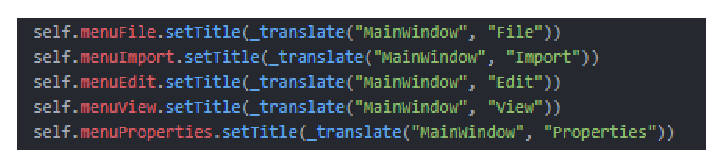
\includegraphics[scale= 1]{intersting-code-2.eps}
  \caption{Python code of renaming the menu bar}
\end{figure}

Before using QtDesigner, we initialized and named everything in the same function.
Our code has generally has some cool implementation parts. There are lots of neat little small tricks in python to be able to design the UI in the way that one wants.

\begin{verbatim}w.setWindowFlags(QtCore.Qt.FramelessWindowHint) 
\end{verbatim}
The above line of code is a good example of how neat the python UI code can be. This snippet of code allows our program to remove the default boarder around the program and implement our own boarder.


\section{Description of First User Study}
We are waiting on our integration team to integrate the GUI and our ArcGIS project. No user study has been conducted yet.
When our project is integrated, we will conduct a user study. In this study we will have user's evaluate our GUI and see if there are any clarity improvements that could be made. 

\renewcommand\refname{Bibliography}

% bibliography
\pagebreak
\nocite{*}%if nothing is referenced it will still show up in refs
\bibliographystyle{IEEEtran}
\bibliography{refs}

%\end{singlespace}
\end{document}